\documentclass[supercite]{Experimental_Report}

\title{~~~~~~新生实践课~~~~~~}
\author{毕梓康}
%\coauthor{张三、李四}
\school{计算机科学与技术学院}
\classnum{2405}
\stunum{U202414652}
%\costunum{U202115631、U202115631}
\instructor{陈加忠} % 该系列实验报告模板由华科大计院教师陈加忠制作
\date{2024年11月20日}

\usepackage{algorithm, multirow}
\usepackage{algpseudocode}
\usepackage{amsmath}
\usepackage{amsthm}
\usepackage{framed}
\usepackage{mathtools}
\usepackage{subcaption}
\usepackage{xltxtra} %提供了针对XeTeX的改进并且加入了XeTeX的LOGO, 自动调用xunicode宏包(提供Unicode字符宏)
\usepackage{bm}
\usepackage{tikz}
\usepackage{tikzscale}
\usepackage{pgfplots}
%\usepackage{enumerate}
\usepackage{geometry} % 用于设置页面布局
\pgfplotsset{compat=1.16}
\newcommand{\cfig}[3]{
  \begin{figure}[htb]
    \centering
    \includegraphics[width=#2\textwidth]{images/#1.tikz}
    \caption{#3}
    \label{fig:#1}
  \end{figure}
}

\newcommand{\sfig}[3]{
  \begin{subfigure}[b]{#2\textwidth}
    \includegraphics[width=\textwidth]{images/#1.tikz}
    \caption{#3}
    \label{fig:#1}
  \end{subfigure}
}

\newcommand{\xfig}[3]{
  \begin{figure}[htb]
    \centering
    #3
    \caption{#2}
    \label{fig:#1}
  \end{figure}
}

\newcommand{\rfig}[1]{\autoref{fig:#1}}
\newcommand{\ralg}[1]{\autoref{alg:#1}}
\newcommand{\rthm}[1]{\autoref{thm:#1}}
\newcommand{\rlem}[1]{\autoref{lem:#1}}
\newcommand{\reqn}[1]{\autoref{eqn:#1}}
\newcommand{\rtbl}[1]{\autoref{tbl:#1}}

\algnewcommand\Null{\textsc{null }}
\algnewcommand\algorithmicinput{\textbf{Input:}}
\algnewcommand\Input{\item[\algorithmicinput]}
\algnewcommand\algorithmicoutput{\textbf{Output:}}
\algnewcommand\Output{\item[\algorithmicoutput]}
\algnewcommand\algorithmicbreak{\textbf{break}}
\algnewcommand\Break{\algorithmicbreak}
\algnewcommand\algorithmiccontinue{\textbf{continue}}
\algnewcommand\Continue{\algorithmiccontinue}
\algnewcommand{\LeftCom}[1]{\State $\triangleright$ #1}

\newtheorem{thm}{定理}[section]
\newtheorem{lem}{引理}[section]

\colorlet{shadecolor}{black!15}

\theoremstyle{definition}
\newtheorem{alg}{代码}[section]

\def\thmautorefname~#1\null{定理~#1~\null}
\def\lemautorefname~#1\null{引理~#1~\null}
\def\algautorefname~#1\null{算法~#1~\null}

\begin{document}

\maketitle

\clearpage

\pagenumbering{Roman}

\tableofcontents[level=2]

\clearpage

\pagenumbering{arabic}

\section{网页整体框架}

当我知道我能够做一个属于自己的网页时,我脑海中第一个浮现的却是小时候看的一本无字图书<<长长的路>>。

我知道这听起来很奇怪,但是,网页对于我来说是一扇通向未知,新奇和幻想的大门,而这些正是这本图书在我小时给予我的。所以,我的网页背景均是这本图书的插画,从过去,现在,未来三方面俯瞰自己。

图1-1展示了页面的测此逻辑,对应于主页wangye.html以及其他的子网页文件

\begin{figure}[htb] % here top bottom
	\begin{center}
		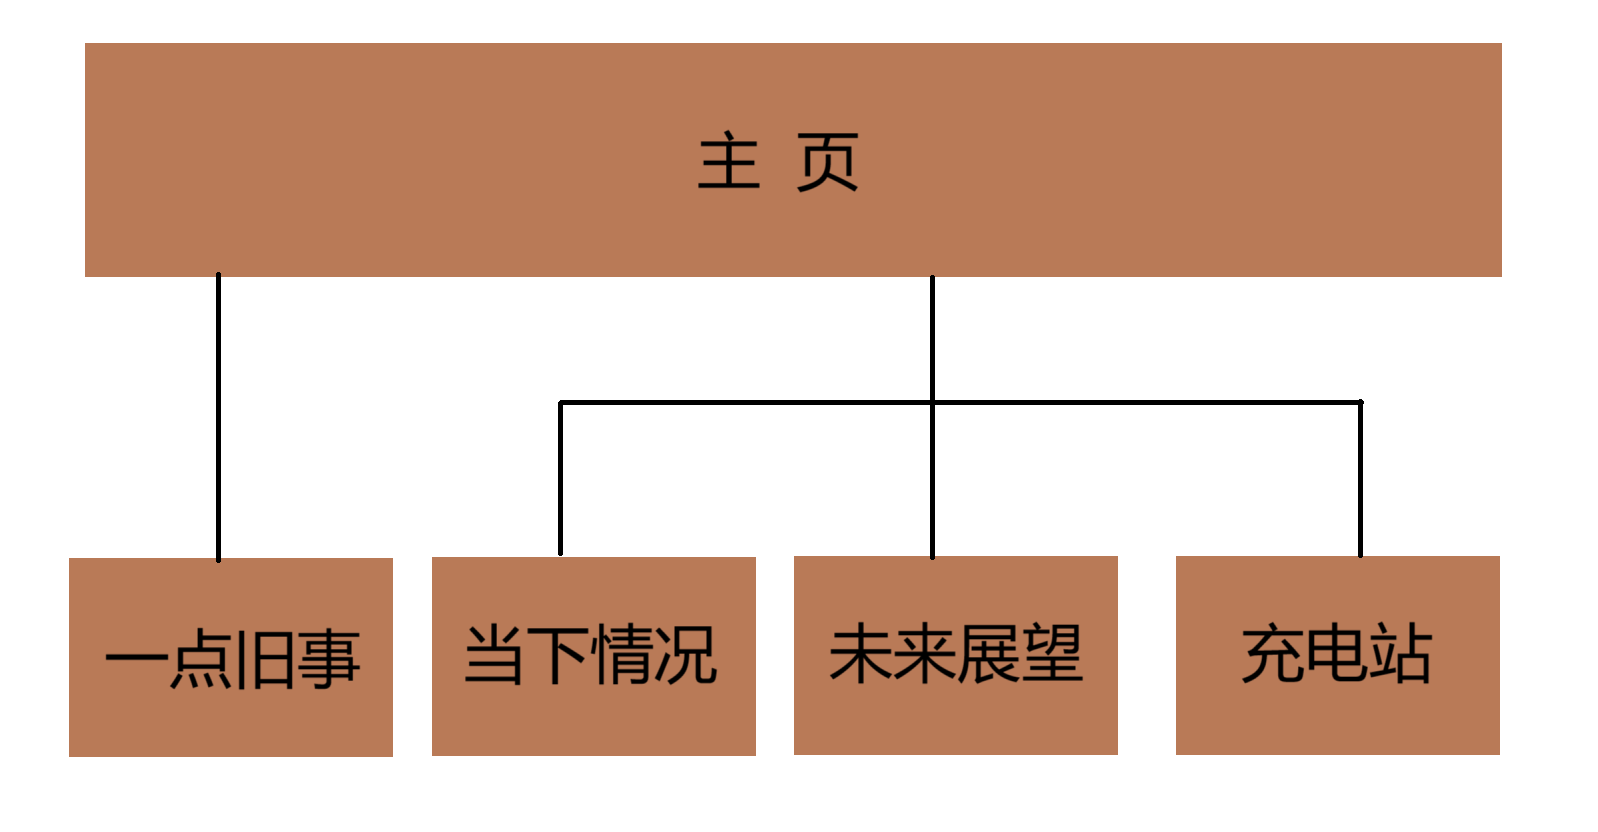
\includegraphics[scale=0.30]{images/1-1.png}
		\caption{我的网页架构}
		\label{fig1-1}
	\end{center}
\end{figure}

从主页开始可以任意进入四个分页,四个分页也可以互相跳转,但主页无法再次到达,因为主页有强制的一段“动画”,访问的用户看两次大概会不耐烦。

总的来说,全部网页主要包括了一下元素:
\begin{enumerate}[label=(\arabic*)]
	\item 主页-毕梓康的主页
	\item 分页面一:一点旧事
	\item 分页面二:当下情况
	\item 分页面三:未来展望
	\item 分页面四:充电站
	\item 其他元素:时钟和音乐
	% 继续添加其他元素
\end{enumerate}

\newpage

\section{个人网页主页设计}
我的主页看起来并不复杂,但实际上设计的时间很久,每个细节都费了不少功夫。

\begin{figure}[htb] % here top bottom
	\begin{center}
		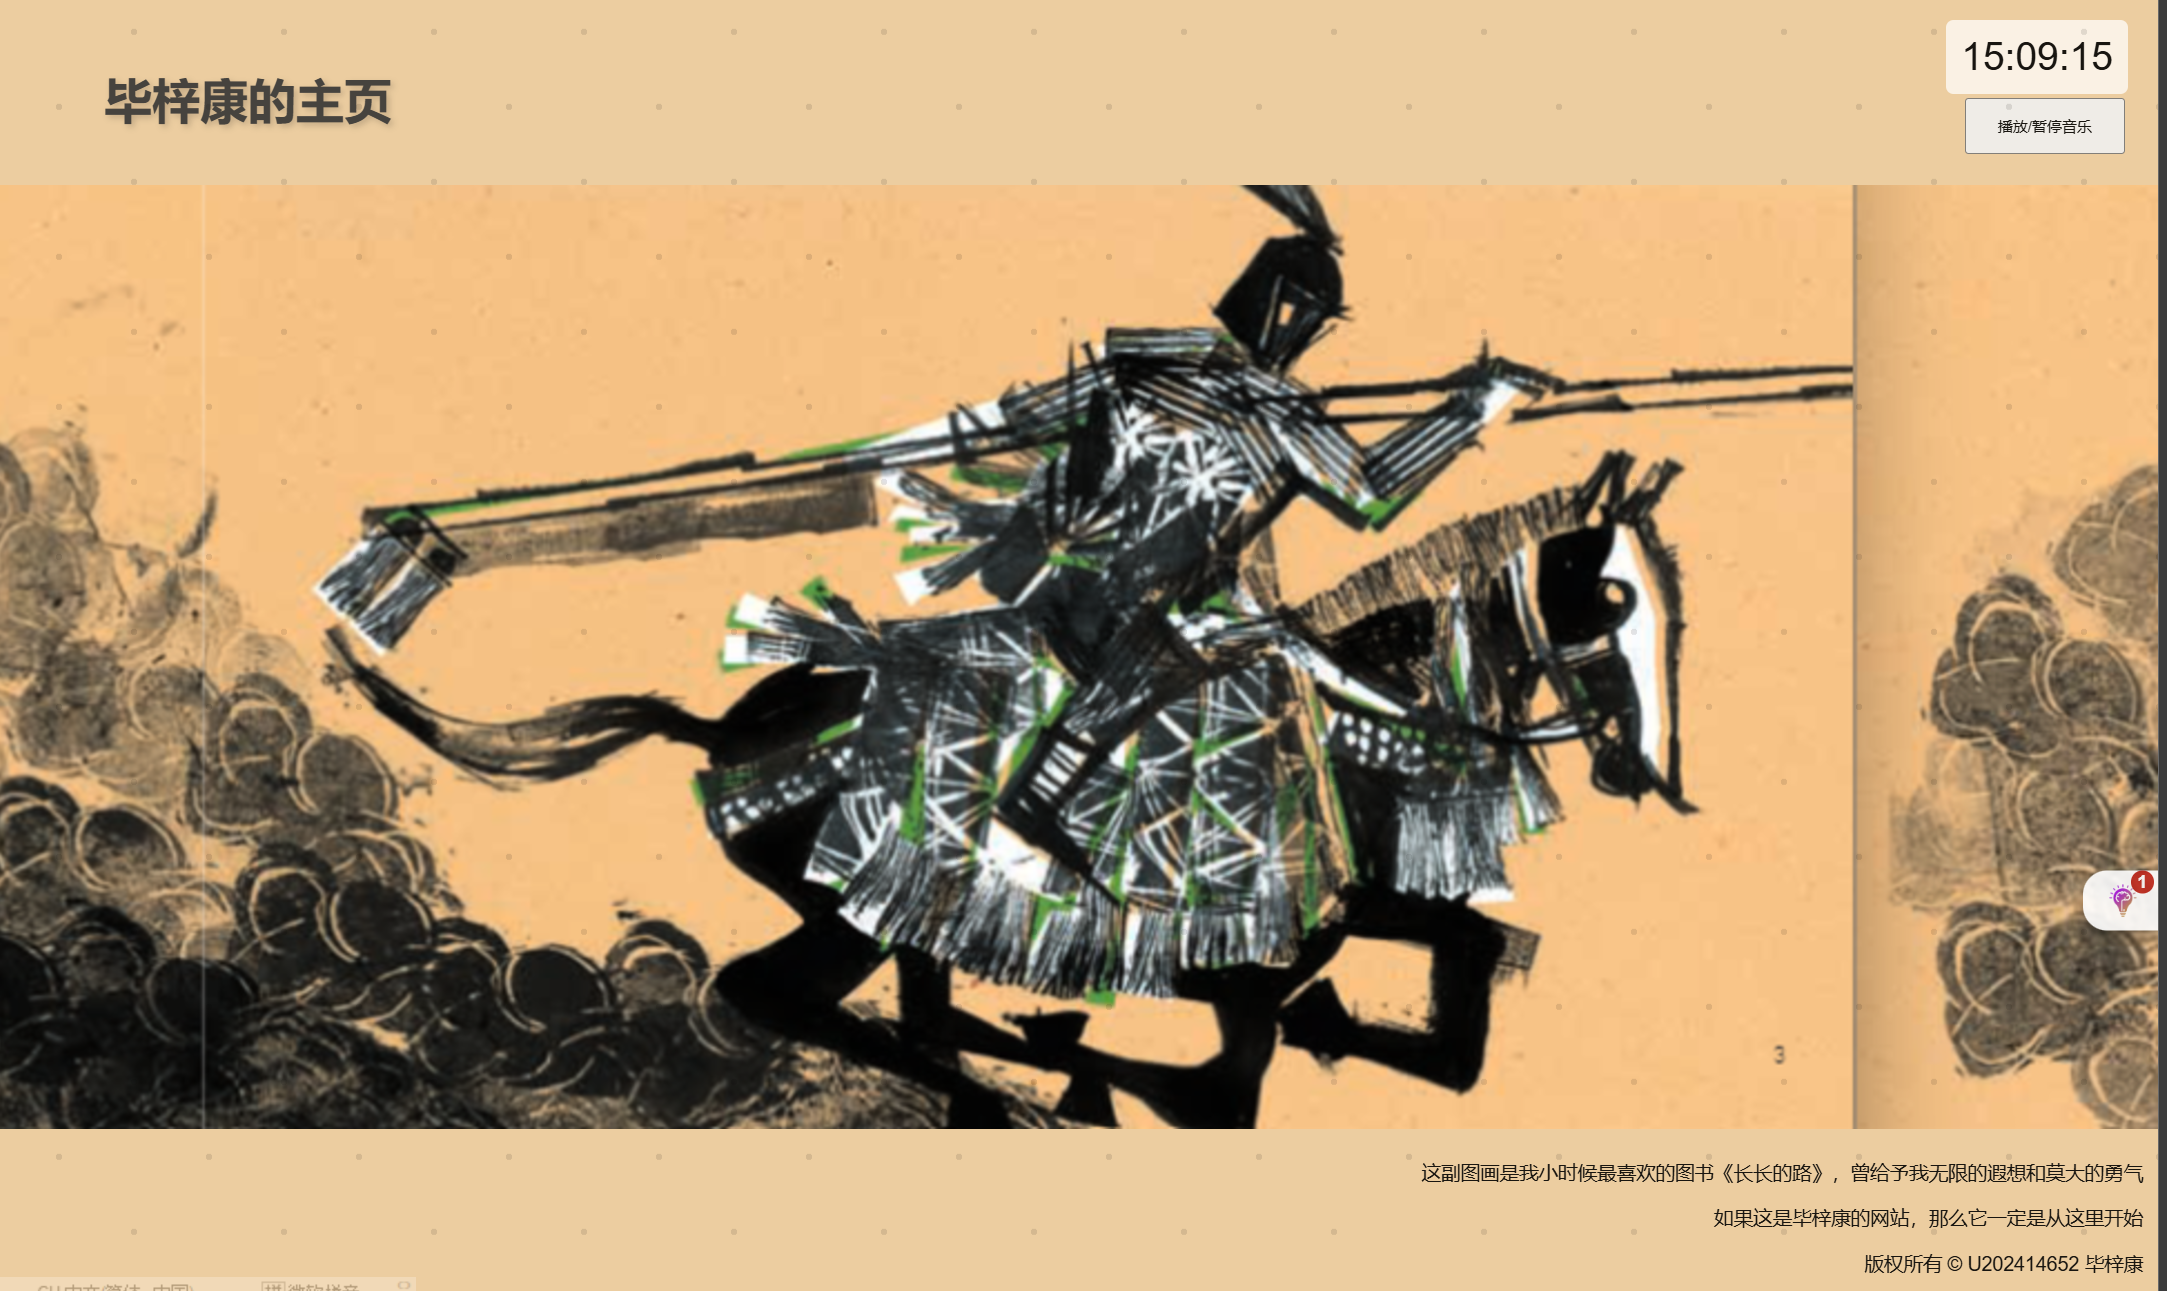
\includegraphics[scale=0.40]{images/zhuye.png}
		\caption{主页}
		\label{fig2-1}
	\end{center}
\end{figure}

整体可以分为四个部分:动态图画,淡入淡出的文字,链接,以及灰尘下落动画

\subsection{动态图画}

最初其实是静态的,但是如果要访问者在链接浮现之前一直盯着不动的画面实在不太合适。于是就想办法改成了动态的。

\begin{figure}[htb] % here top bottom
	\begin{center}
		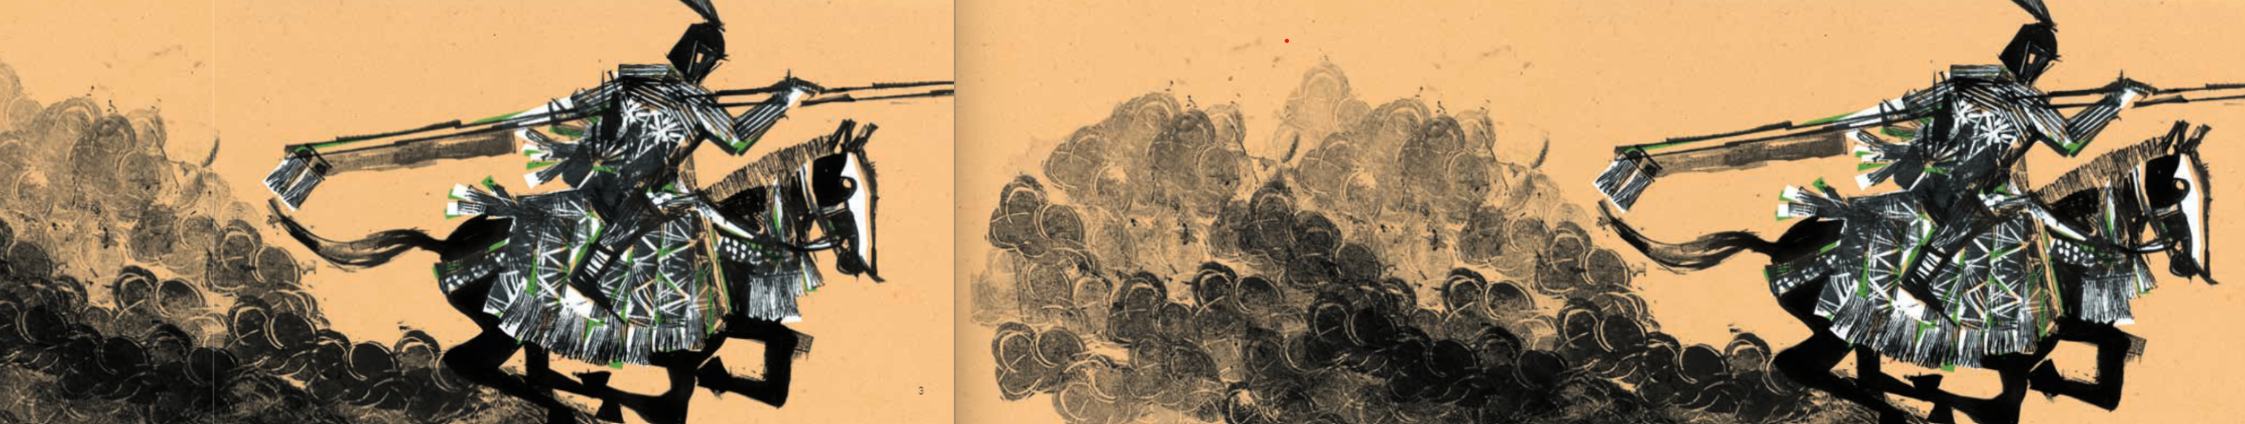
\includegraphics[scale=0.40]{images/zhuye-1.png}
		\caption{真实的背景图}
		\label{fig2-2}
	\end{center}
\end{figure}


如图所示这个动态的效果实际上是一个两倍长的图画从左到右移动,移动到最左侧再再次回到右侧,重新开始新一轮的移动
\begin{verbatim}
	@keyframes slideBackground {
		from {
			background-position: 0 130px; /* 从最左边开始 */
		}
		to {
			background-position: 100% 130px; /* 移动到最右边 */
		}
	}
\end{verbatim}
很简单的实现,但是效果却非常好

\subsection{文字的淡入淡出}

我并不打算占用这个页面,那样会使得我的我也看起来很臃肿。而且我也希望浏览者能有时间好好欣赏这幅图画,所以我设计了右下角淡入有淡出的文字,以及之后会慢慢浮现的链接。
\begin{figure}[htb] % here top bottom
	\begin{center}
		
\includegraphics[scale=0.80]{images/zhuye-2.png}
		\caption{开始时}
		\label{fig2-3}
	\end{center}
\end{figure}

\begin{figure}[htb] % here top bottom
	\begin{center}
		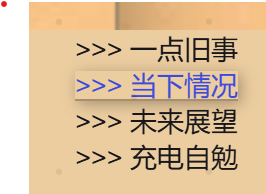
\includegraphics[scale=0.80]{images/zhuye-3.png}
		\caption{结束时}
		\label{fig2-4}
	\end{center}
\end{figure}


代码上比较复杂,用到了两个函数
\begin{verbatim}
	@keyframes fadeIn {
		from { opacity: 0; }
		to { opacity: 1; }
	}
	@keyframes fadein-outText {
		0%, 100% { opacity: 0; } /* 开始和结束时透明度为0 */
		20%, 80% { opacity: 1; } /* 中间部分透明度为1 */
	}
\end{verbatim}

一个是标题和之后的链接通用的淡入fadein 和为了出现又消失的文字单独设置的动画fadein-outText
这是我最喜欢的一块设计,实际上实现起来并不是很麻烦,但是调各个时间点不容易
\subsection{链接}
我为介绍之后浮现的链接增加了鼠标悬停效果,让其看上去更有设计感。

\begin{figure}[htb] % here top bottom
	\begin{center}
		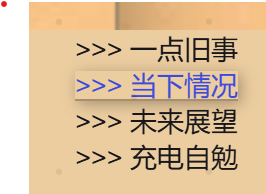
\includegraphics[scale=0.40]{images/zhuye-3.png}
		\caption{对,又是这张图}
		\label{fig2-5}
	\end{center}
\end{figure}

部分代码如下,并没有什么好说的,实际实现其实蛮复杂的

\begin{verbatim}
a:hover {
	color: #3c4add; /* 悬停时颜色加深 */
	box-shadow: 2px 2px 10px rgba(0, 0, 0, 0.3); /* 添加阴影 */
	transition: box-shadow 0.3s ease; 
}

/* 阴影效果 */
a::after {
	content: '';
	position: absolute;
	bottom: 0;
	left: 0;
	right: 0;
	margin: auto;
	height: 1px; 
	background: rgba(0, 0, 0, 0.3); 
	opacity: 0; /* 初始透明度为0 */
	transition: opacity 0.3s ease; /* 平滑过渡*/
}

/* 链接悬停时显示阴影 */
a:hover::after {
	opacity: 1; 
}
\end{verbatim}

\subsection{灰尘下落动画}
最费时间的一段,本来希望设法增加灰尘的数量和随机化下落轨迹,遭遇了悲惨的失败,于是改为简单的下落半透明黑点

因为太过写意一度被室友当成是黑色的雪,不过也挺浪漫的不是吗

\begin{figure}[htb] % here top bottom
	\begin{center}
		
\includegraphics[scale=0.40]{images/zhuye-4.png}
		\caption{请您仔细看}
		\label{fig2-6}
	\end{center}
\end{figure}
欸,太透明就不好注意到,太明显又妨碍阅读,只好取这种折中的效果

照例,部分代码,其实主要实现是后边的一段,太长了不适合放在这个报告中
\begin{verbatim}
	@keyframes dustFall {
		0% {
			transform: translateY(-5px);
			opacity: 0;
		}
		50% {
			opacity: 0.5;
		}
		100% {
			transform: translateY(105vh);
			opacity: 0;
		}
	}
\end{verbatim}

这四个操作在子页面之中也会用到,将不再次赘述

\newpage

\section{分页面1-一点旧事}
四个分页面的背景其实是图画书中骑士故事的四节,一脉相承又各有蕴意,此页面背景是骑士最初的传奇经历,代表我的过去
\begin{figure}[htb]
	\begin{center}
		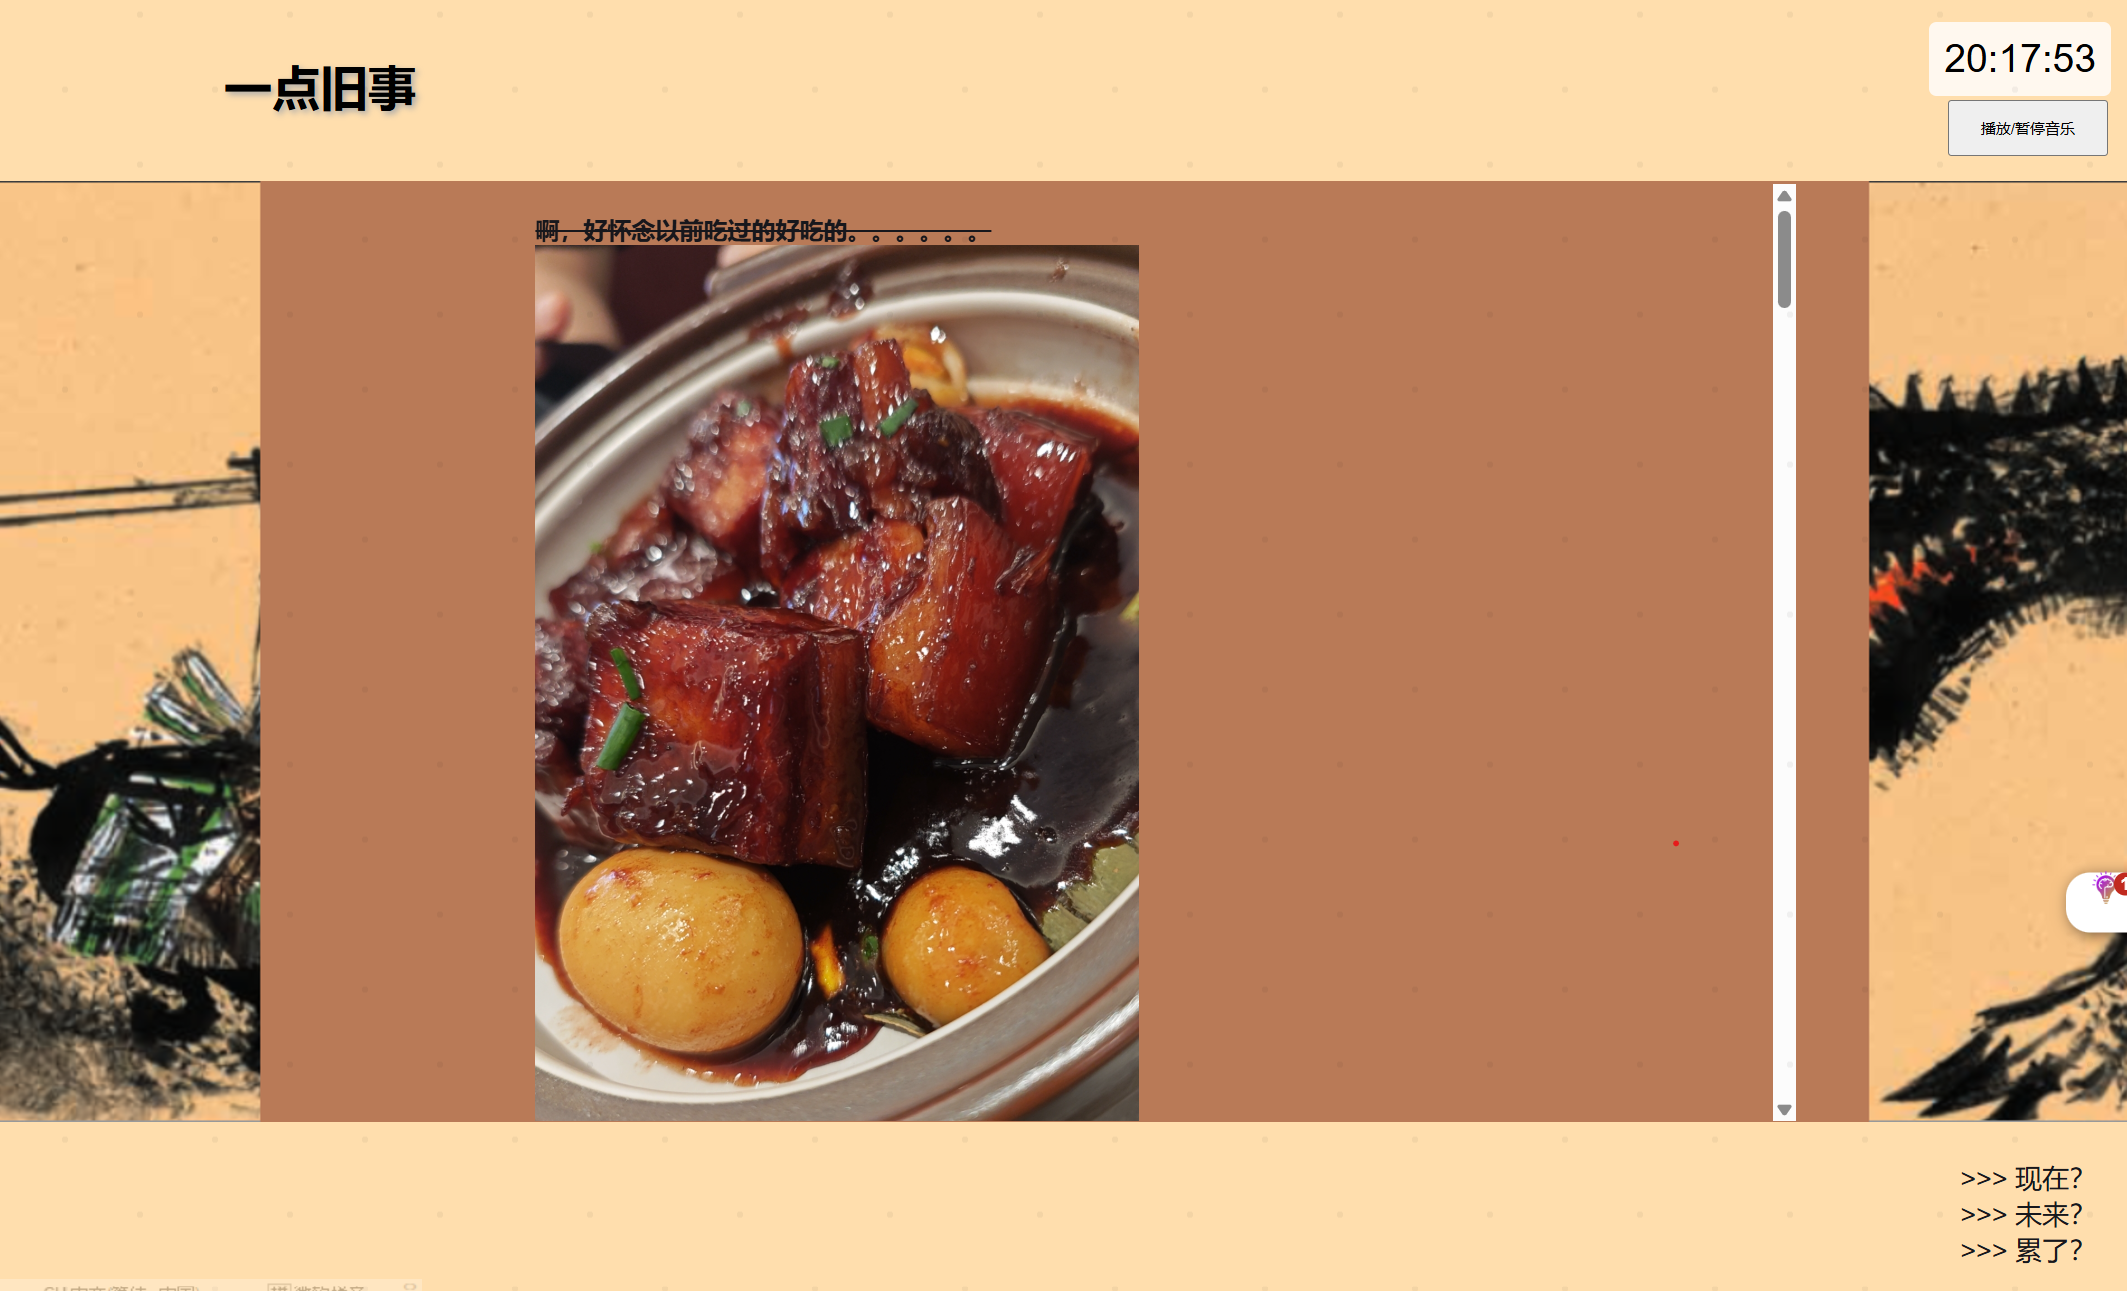
\includegraphics[scale=0.40]{images/jiushi-1.png}
		\caption{一点旧事}
		\label{fig3-1}
	\end{center}
\end{figure}
从内容方面,这个文本回忆了我过去的美好回忆。

显然可以看出这个页面和上个页面有很多相似的设计和大量的挪用,但还是有一些值得注意的地方

而且因为背景图片的高度不统一,我不得不每个页面手动调整链接和标题的出现位置以及内边距,实际上是一份无聊又麻烦的工作
\subsection{字符逐个出现}

我希望汉字能够逐个出现,而不是一起蹦出来,毕竟我希望网页与网页之间的衔接不要太突兀,于是就制作了这个效果
\begin{figure}[htb]
	\begin{center}
		
\includegraphics[scale=0.40]{images/3-2.png}
		\caption{效果图}
		\label{fig3-2}
	\end{center}
\end{figure}
\begin{verbatim}

const letters = document.querySelectorAll('.text-block span');
let letterIndex = 0;
function typeLetter() {
	if (letterIndex < letters.length) {
		letters[letterIndex].style.opacity = 1;
		letterIndex++;
		setTimeout(typeLetter, 100); // 100毫秒显示一个字符
	}
}

\end{verbatim}

哇,这么简单的操作一定很好完成吧,但是其实这个办法需要每个字符前后加上<span></span>,而我又码了相当多的汉字,所以代码就要很长

\begin{figure}[htb]
	\begin{center}
		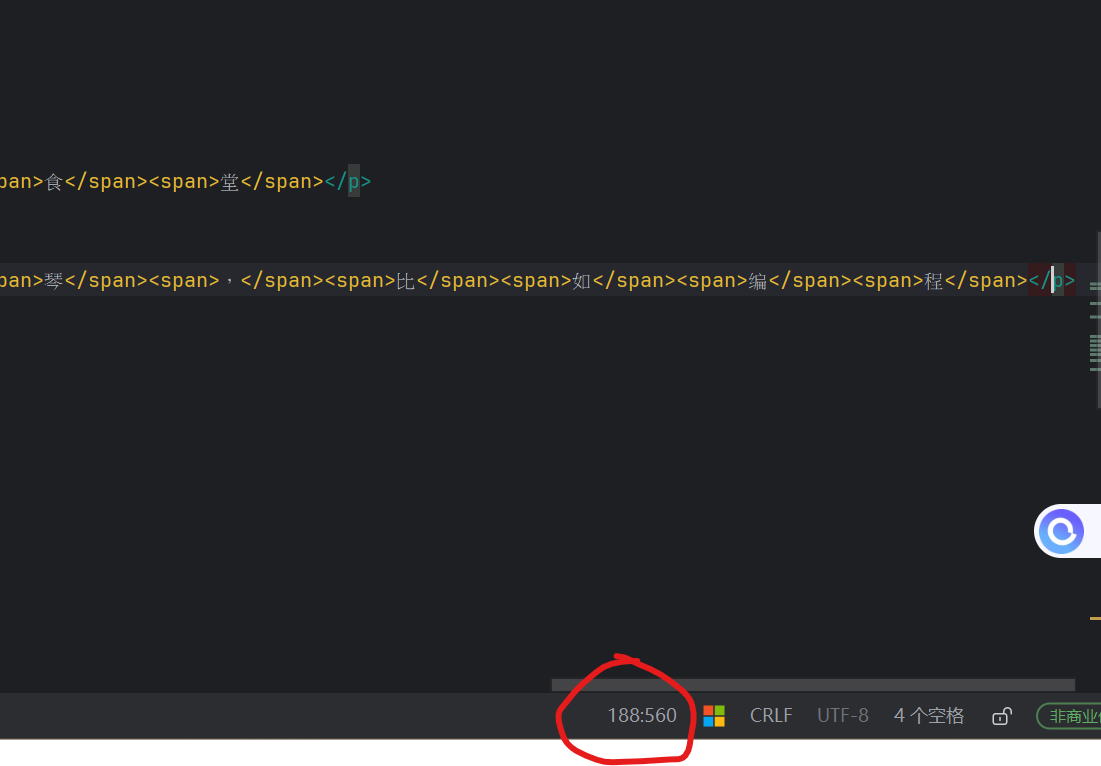
\includegraphics[scale=0.40]{images/3-3.png}
		\caption{瞧瞧这个长度}
		\label{fig3-3}
	\end{center}
\end{figure}
\subsection{滚动条}
我希望做出页面嵌套页面的效果,所以制作选取了页面的一部分展示文本,并制作了滚动条
\begin{figure}[htb]
	\begin{center}
		
\includegraphics[scale=0.40]{images/3-4.png}
		\caption{效果图}
		\label{fig3-4}
	\end{center}
\end{figure}
这段代码就是中间的文本主体
\begin{verbatim}
	
 .content {
	position: absolute;
	top: 113px; 
	right: 30px; /* 这两个数都是慢慢调出来的*/
	color: #17171c;
	z-index: 100;
	width: 70%; /* 内容宽度 */
	max-height: 74vh; /* 最大高度 */
	overflow-y: scroll; /* 显示滚动条 */
	padding: 20px; /* 添加内边距 */
	box-sizing: border-box; 
	font-weight: bold; /* 字体加粗 */
}
\end{verbatim}
除了这两点之外,我还在这几个子网页中加入了大量的图片,相似的操作在后文不再赘述
\newpage
\section{分页面2-当下情况}

此页面背景是骑士损失战马却收服巨龙,踏上更高的层次,代表我的当下

\begin{figure}[htb]
	\begin{center}
		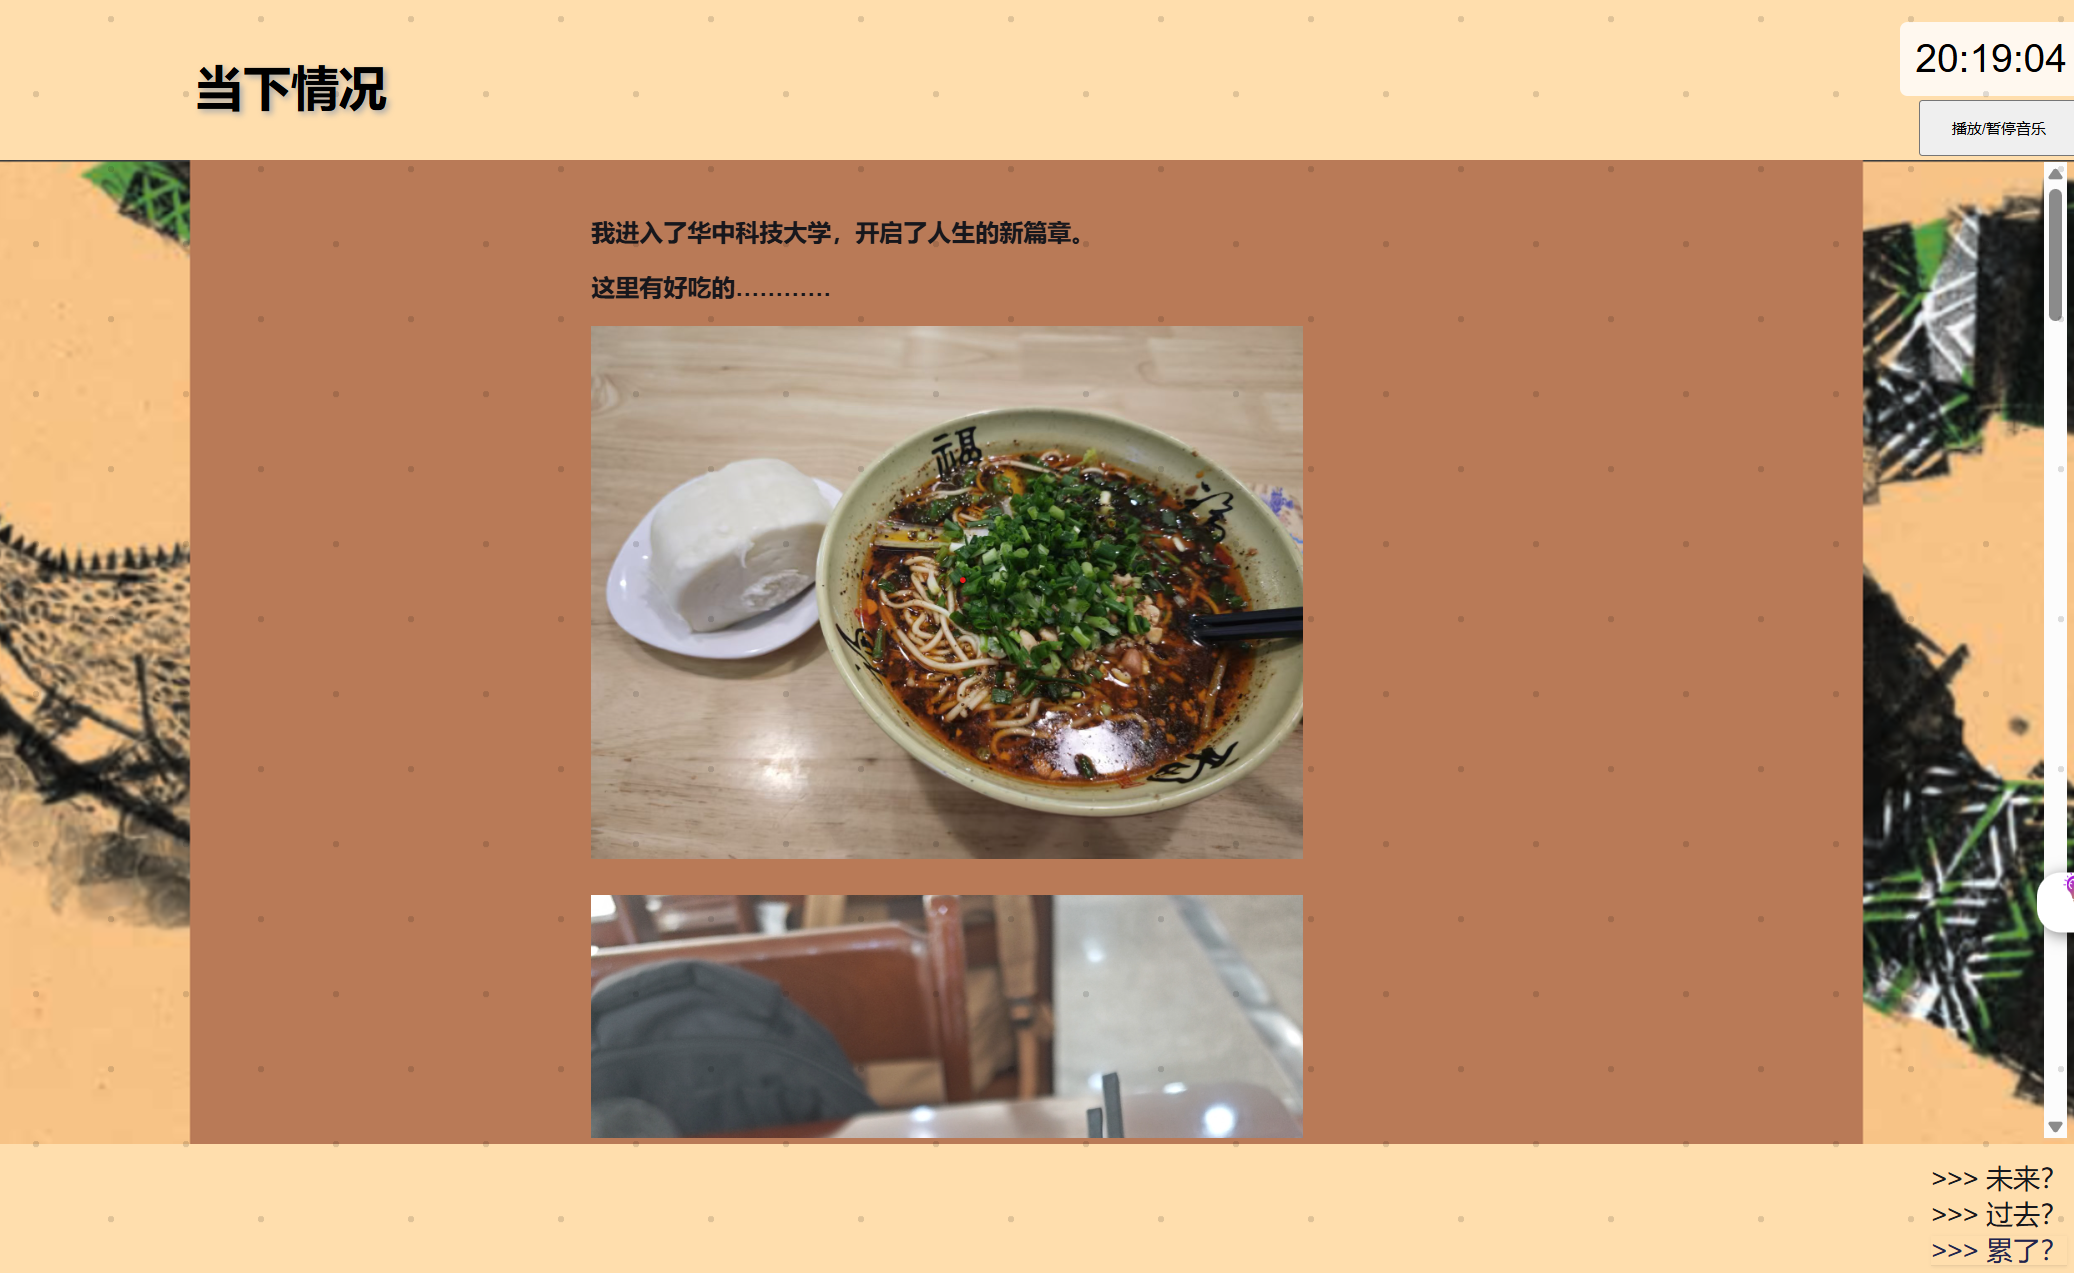
\includegraphics[scale=0.40]{images/dangxia-1.png}
		\caption{当下情况}
		\label{fig4-1}
	\end{center}
\end{figure}
这一页面与“一点旧事”在结构上并无差别

内容上,这一页面从吃住,学习,交友等方面介绍了当下的生活,之后发给爸爸妈妈看,他们也会放心

我发现我真的挺爱吃,手机里的图片有相当一部分都是美食,也是这个页面的素材来源。

\newpage
\section{分页面3-未来展望}

此页面是骑士与他的伙伴巨蛇一起冲破重重困难,勇敢向前,代表我的未来

\begin{figure}[htb]
	\begin{center}
		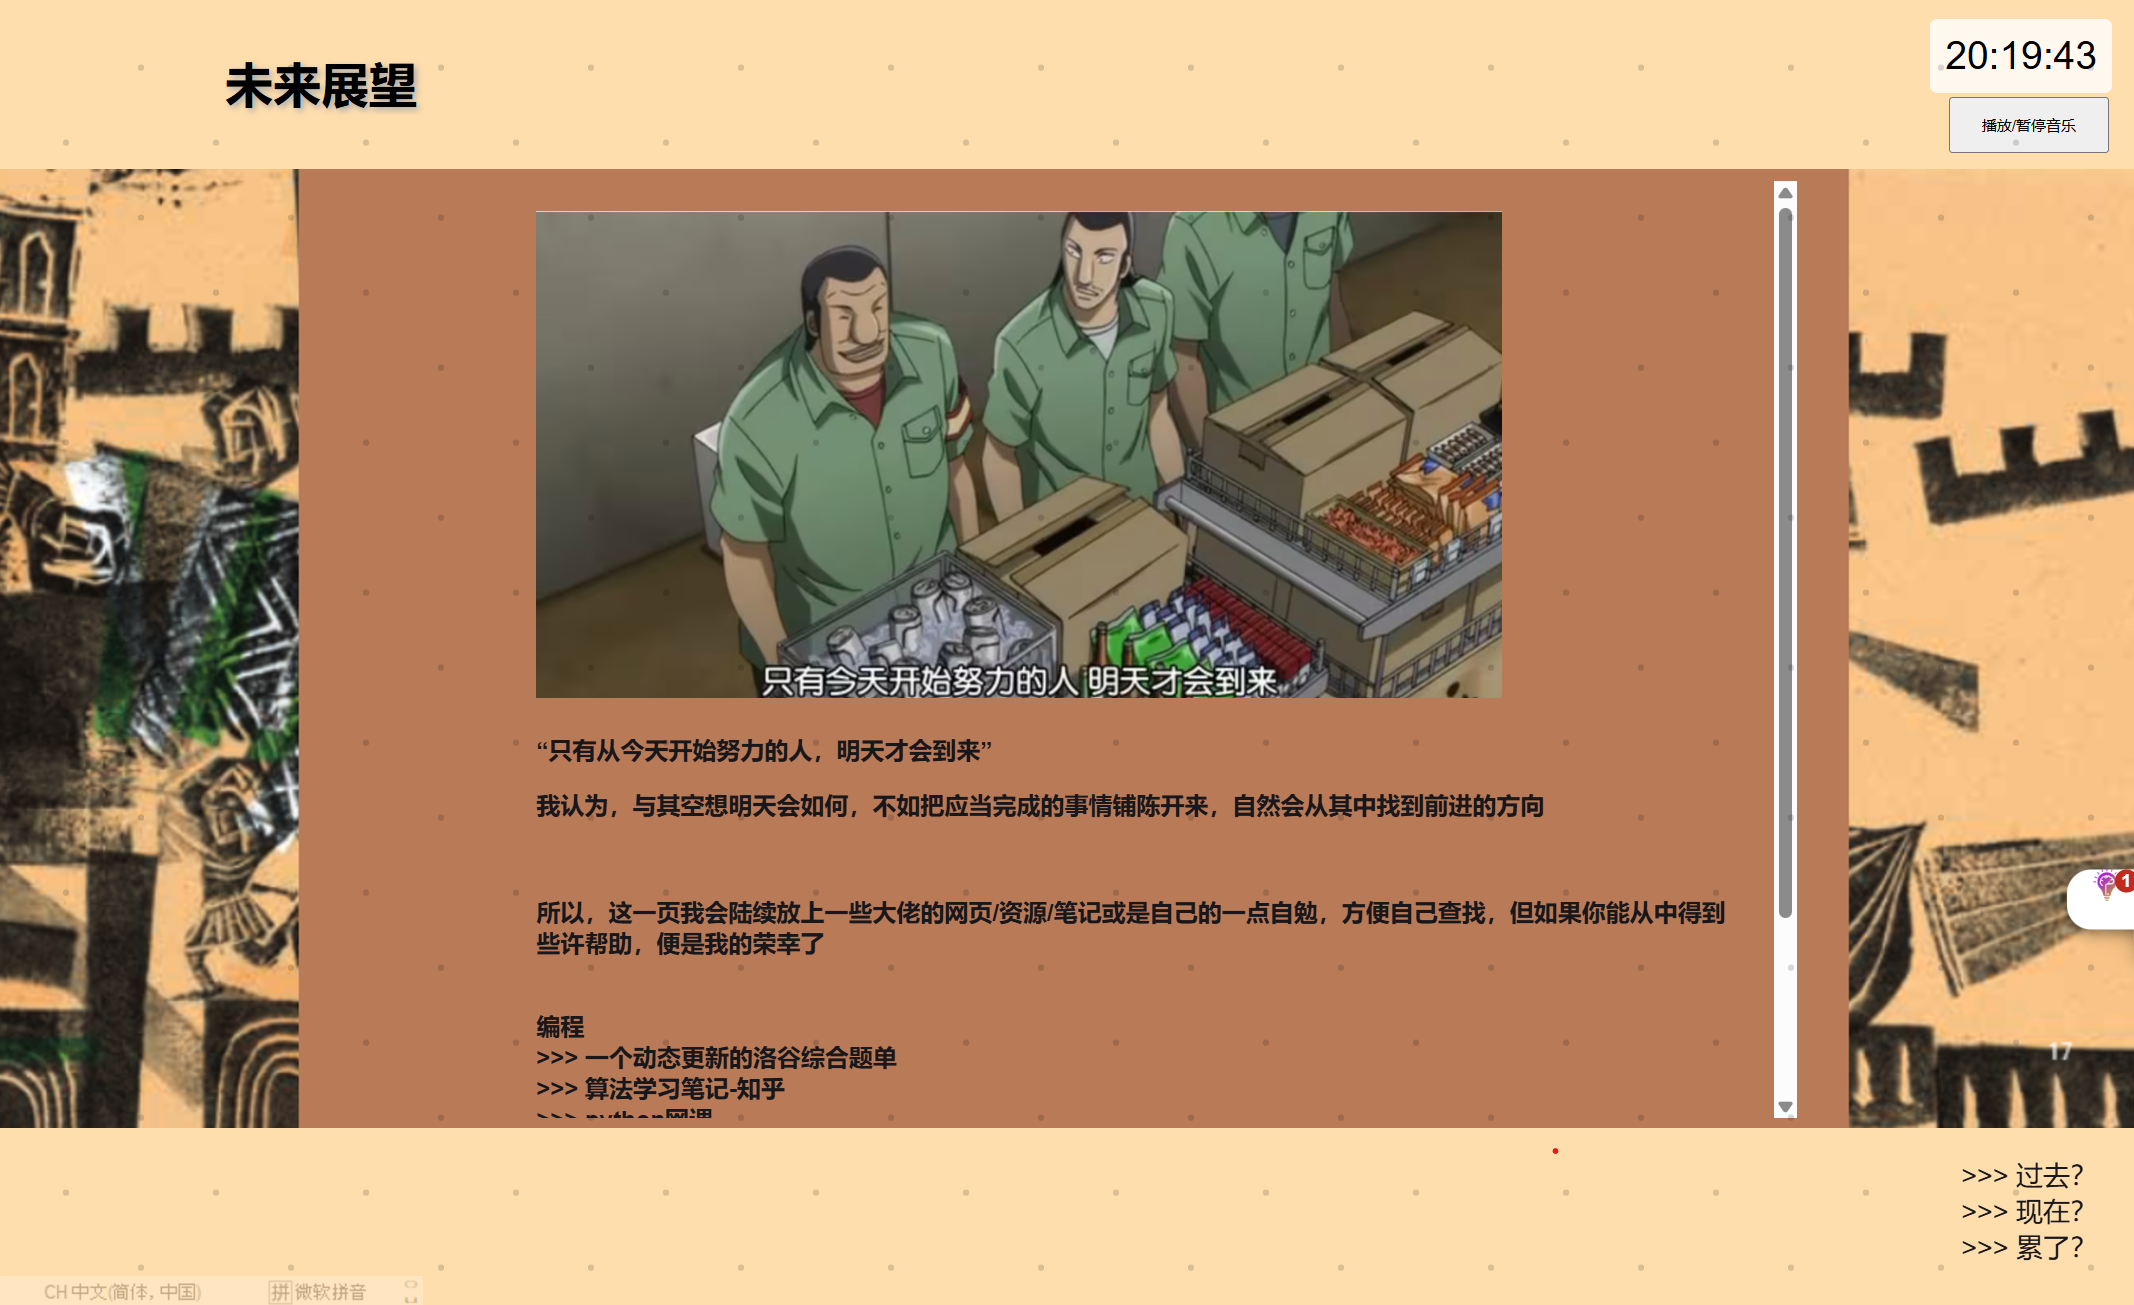
\includegraphics[scale=0.40]{images/weilai-1.png}
		\caption{未来展望}
		\label{fig5-1}
	\end{center}
\end{figure}

这个页面是不是看上去挺简洁的

我觉得自己的网站不应该失去实用性,于是在这个页面放上了一些自己能用得上,或许还对其他人有帮助的东西。

现在东西还不是很多,不过以后我会继续维护的。

另外,图片来自动漫<<赌博默示录>>,很好的动漫,有教育意义。

\newpage
\section{充电站}

谁都有没劲的时候,不是吗,我希望自己累的时候能从这个网站里打打气,就像背景中的骑士不断的前进,攀登

所以我设计了这个页面,并取名为充电站

这些书其实是我上大学之后才开始读的,高中没时间,我都不知道自己其实挺喜欢读书的

\begin{figure}[htb]
	\begin{center}
		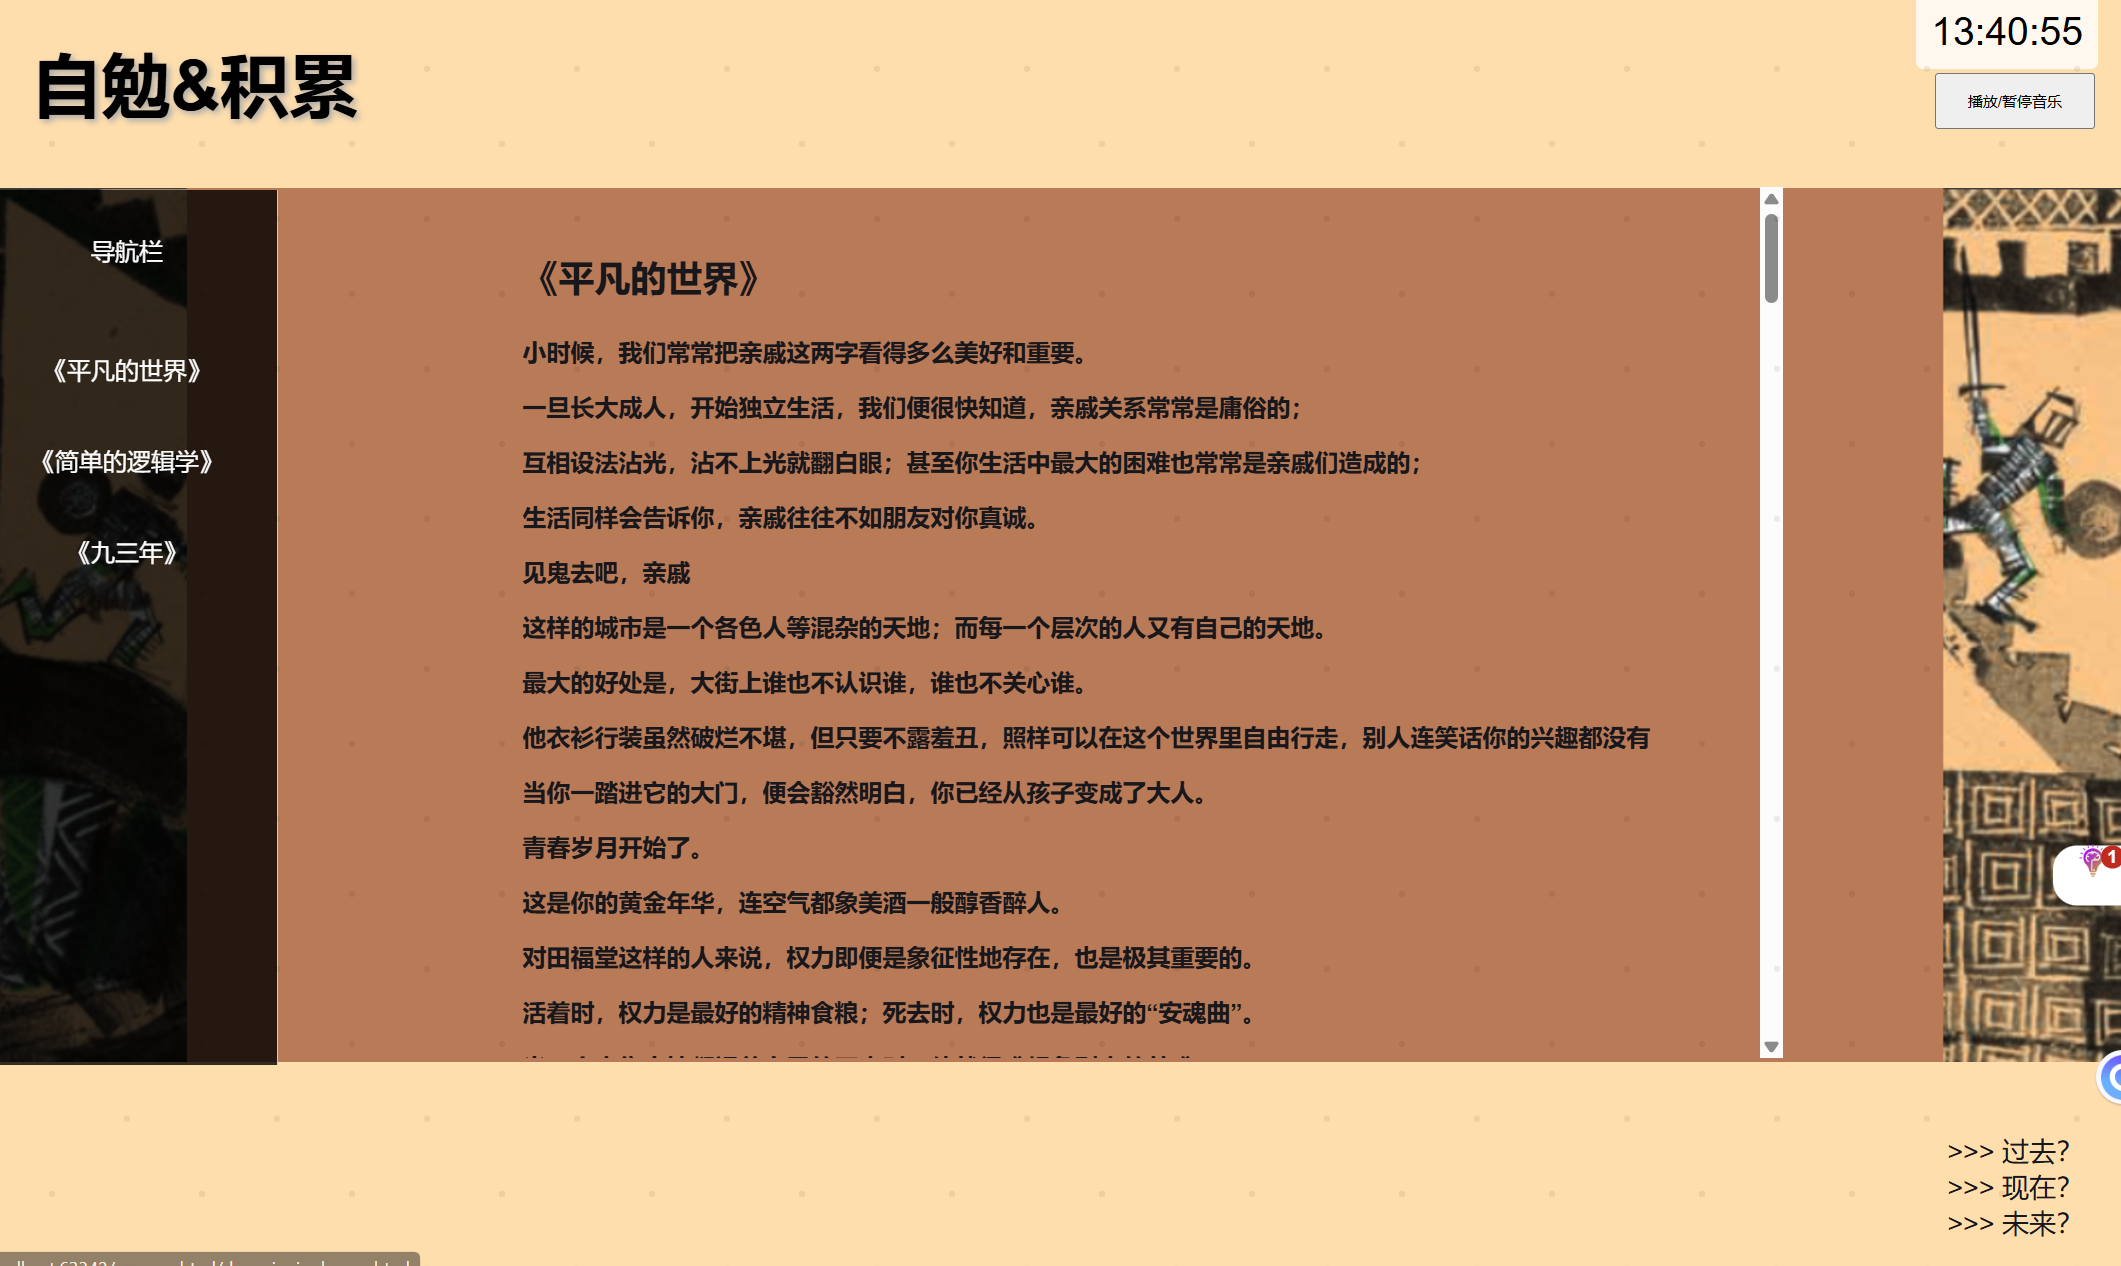
\includegraphics[scale=0.40]{images/6-1.png}
		\caption{充电站}
		\label{fig6-1}
	\end{center}
\end{figure}

这个页面与另外几个分页面不一样,文本量很大,所以设计了侧边导航栏让读者能快速找到自己想浏览的段落
\begin{figure}[htb]
	\begin{center}
		
\includegraphics[scale=0.40]{images/6-2.png}
		\caption{click}
		\label{fig6-2}
	\end{center}
\end{figure}

嗯,以后大概还会加入其他的书籍摘抄,希望有一天这里能变成我的小书库

代码实现是通过给每段摘抄增加一个类来做的herf来做的,nav的代码这里就不再放了

\newpage
\section{其他-音乐和时钟}

功能性部件,每个页面均有这两个东西。
\begin{figure}[htb]
	\begin{center}
		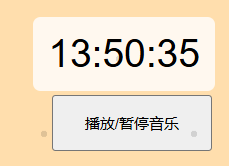
\includegraphics[scale=0.40]{images/7-1.png}
		\caption{clock and music}
		\label{fig7-1}
	\end{center}
\end{figure}

音乐本来是默认播放的,后来想到默认播放很容易吓到浏览者就改成默认关闭了

按钮文本会随着当前状态放生变化
\begin{figure}[htb]
	\begin{center}
		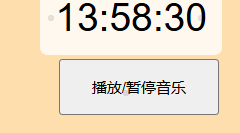
\includegraphics[scale=0.40]{images/7-2.png}
		\caption{初始状态}
		\label{fig7-2}
	\end{center}
\end{figure}

\begin{figure}[htb]
\begin{center}
	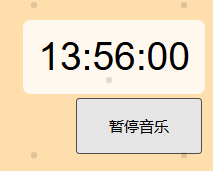
\includegraphics[scale=0.40]{images/7-3.png}
	\caption{另一个状态}
	\label{fig7-3}
\end{center}
\end{figure}

给出代码:
\begin{verbatim}
	
toggle.addEventListener('click', function() {
	if (audio.paused) {
		audio.play();
		toggle.textContent = '暂停音乐';
	} else {
		audio.pause();
		toggle.textContent = '播放音乐';
	}
});
\end{verbatim}

\newpage

\apendix

\section{写在最后}
其实每个页面的头文本都是不一样的,不过太中二了,我都不好意思在这个实验报告的正文提
\begin{figure}[htb] % 将所有图片放在一个figure环境中
	\centering
	\begin{subfigure}[b]{0.4\textwidth}
		
\includegraphics[width=\textwidth]{images/e1.png}
		\caption{主页}
		\label{fig8-1}
	\end{subfigure}
	\hfill % 添加一些水平间距
	\begin{subfigure}[b]{0.4\textwidth}
		
\includegraphics[width=\textwidth]{images/e2.png}
		\caption{一点旧事}
		\label{fig8-2}
	\end{subfigure}
	
	\begin{subfigure}[b]{0.4\textwidth}
		
\includegraphics[width=\textwidth]{images/e5.png}
		\caption{当下情况}
		\label{fig8-3}
	\end{subfigure}
	\hfill
	\begin{subfigure}[b]{0.4\textwidth}
		
\includegraphics[width=\textwidth]{images/e6.png}
		\caption{未来展望}
		\label{fig8-4}
	\end{subfigure}
	
	\begin{subfigure}[b]{0.4\textwidth}
		
\includegraphics[width=\textwidth]{images/e7.png}
		\caption{充电站}
		\label{fig8-5}
	\end{subfigure}
\end{figure}
\end{document}